\documentclass[a4paper]{scrreprt}


%%% PACKAGES %%%

% add unicode support and use german as language
\usepackage[utf8]{inputenc}
\usepackage[ngerman]{babel}

% Use Helvetica as font
\usepackage[scaled]{helvet}
\renewcommand\familydefault{\sfdefault}
\usepackage[T1]{fontenc}

% Better tables
\usepackage{tabularx}

% Better enumerisation env
\usepackage{enumitem}

% Use graphics
\usepackage{graphicx}


% Have custom abstract heading
\usepackage{abstract}

% Need a list of equation
\usepackage{tocloft}
\usepackage{ragged2e}

% Better equation environment
\usepackage{amsmath}

% Symbols for most SI units
\usepackage{siunitx}

\usepackage{csquotes}

% Clickable Links to Websites and chapters
\usepackage{hyperref}

% Symbols like checkmark
\usepackage{amssymb}

% Bibliography & citing
\usepackage[
	backend=biber,
	style=apa,
	bibstyle=apa,
	citestyle=apa,
	sortlocale=de_DE
	]{biblatex}
\addbibresource{Referenzen.bib}
\DeclareLanguageMapping{ngerman}{ngerman-apa}

%%% COMMAND REBINDINGS %%%
\newcommand{\tabitem}{~~\llap{\textbullet}~~}

% Define list of equations - Thanks to Charles Clayton: https://tex.stackexchange.com/a/354096
\newcommand{\listequationsname}{\huge{Formelverzeichnis}}
\newlistof{myequations}{equ}{\listequationsname}
\newcommand{\myequations}[1]{
	\addcontentsline{equ}{myequations}{\protect\numberline{\theequation}#1}
}
\setlength{\cftmyequationsnumwidth}{2.3em}
\setlength{\cftmyequationsindent}{1.5em}

% Usage {equation}{caption}{label}
\newcommand{\indexequation}[3]{
	\begin{align} \label{#3} \ensuremath{\boxed{#1}} \end{align}
	\myequations{#3} \centering \small \textit{#2} \normalsize \justify }

%%% PATH DEFINITIONS %%%
% Define the path were images are found
\graphicspath{{./img/}{./pdf/}}

%%% TITLEPAGE %%%

\title{Projektdokumentation}
\subtitle{PAWI HS18}
\author{Pascal Baumann, Dane Wicki}
\publishers{Richard Wetzel}
\date{\today}

%%% DOCUMENT %%%

\begin{document}

\begin{titlepage}
\maketitle
\end{titlepage}

\renewcommand{\abstractname}{Management Summary}
\begin{abstract}
	Hier könnte ihr Management Summary stehen.
\end{abstract}

\section*{Versionskontrolle}

\begin{tabularx}{\textwidth}{|c|c|c|X|}
	\hline
	\textbf{Versionsnummer} & \textbf{Kürzel} & \textbf{Datum} & \textbf{Beschreibung} \\
	\hline
	0.1 & PB & 10.09.18 & Erste Versionierung \\
	\hline
\end{tabularx}

\tableofcontents

\chapter{Einführung}

\chapter{Problemstellung und Vision}

Der Projektbeschrieb unserer Arbeit stellt das Problem, welches wir in unserer Arbeit lösen sollten, wie folgt dar:

\vspace{1em}

\textquotedblleft Der Neubau des zukünftigen Informatik-Gebäudes am Bahnhof in Rotkreuz schreitet stetig voran. Passanten und Besucher sehen diesen Rohbau sowie auf den umgebenden Wänden in Form von fotografischen Visualisierungen.
In dieser Arbeit soll untersucht werden, inwiefern das Gebäude mittels Augmented Reality vor Ort selbst dargestellt werden kann, um interessierten Nutzern ein besseres Verständnis des Neubaus zu vermitteln. \textquotedblright

\vspace{1em}

Wir leiteten daraus die folgende Problemstellung ab:

\vspace{1em}

\textbf{\textquotedblleft Wie und mit welchen Geräten können Neubauten in Ortsnähe in Echtzeit visualisiert werden. \textquotedblright}

\vspace{1em}

Aus der Problemstellung wird klar, dass zuerst eine Evaluation geeigneter Geräte, vor allem in Bezug auf den Ausseneinsatz und Verfügbarkeit durchgeführt werden muss. Danach muss für die jeweilige Plattform ein geeignetes AR Framework gefunden oder erstellt werden, und schlussendlich die Applikation selber entwickelt werden.

Unsere Vision war es, dass unsere Arbeit nicht nur für dieses Projekt einen Nutzen haben sollte, sondern auch für die breitere Gesellschaft. So wird momentan bei einem ordentlichen Bauvorhaben in der Schweiz vom Bauherren nach Einreichung des Baugesuchs, sogenannte Bauprofile aufgestellt. Diese sollen einen Überblick über die Dimensionen eines Neubaus geben, sind jedoch inadäquat um ein wirkliches Bild des Gebäudes wiederzugeben. Daher stellten wir uns vor, dass nicht nur diese Bauprofile aufgestellt werden, sondern dass ebenfalls ein Mittel zur Verfügung gestellt wird, den geplanten Neubau mittels Augmented Reality auf dem Grundstück zu sehen.

\chapter{Stand der Forschung}

\section{Technologische Grundlagen}

\subsection{Historische Entwicklung}
Als Augmented Reality (dt. erweiterte Realität) versteht man das Vermitteln von Zusatzinformationen über die Umgebung in Form von Animationen, Einblendungen und Tonwiedergaben. In den meisten Fällen wird dies über Smartphones oder Computer bewerkstelligt, es existieren jedoch auch spezialisierte Geräte wie die Microsoft HoloLens oder Google Glass. Der Term wurde erstmals von \citeauthor{Milgram1994} im Jahre 1994 detailliert definiert, wobei sie die Vermischung der realen und virtuellen Welt betrachten und wohin die Technologie Augmented Reality fällt (siehe \ref{fig:RVContiinum}):

\vspace{1em}

\textquotedblleft the above-mentioned broad definition of Augmented Reality –  \textquoteleft augmenting natural feedback to the operator with simulated cues\textquoteright\ – is quite clear. Also noteworthy in this figure is the corresponding concept of Augmented Virtuality (AV), which results automatically, both conceptually and lexically, from the figure. \textquotedblright\ \parencite{Milgram1994}

\begin{figure}[htb]
	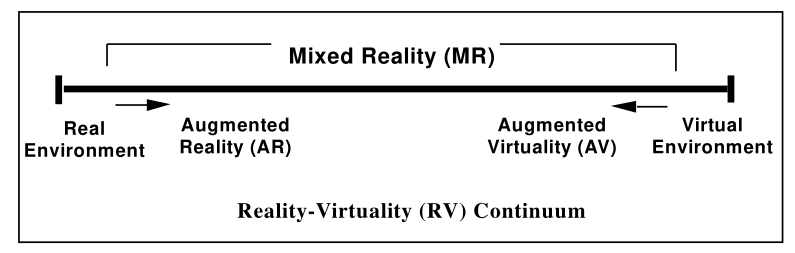
\includegraphics[keepaspectratio, width=\textwidth]{MR_milgram.png}
	\caption{Simplified representation of a RV continuum \parencite{Milgram1994}}
	\label{fig:RVContiinum}
\end{figure}

Fünf Jahre nach Milgram veröffentlichten \citeauthor{Kato1999} ihre Ergebnisse zu einem Marker-basierten AR Konferenzsystem. Sie lösten dabei das Problem der Registrierung (wo befindet sich der Benutzer, oder besser gesagt dessen Augen), und das Ermitteln der Pose (wie ist die Orientierung der virtuellen Kamera in Bezug zur Umwelt) über Marker mit einer fixen Grösse \parencite{Kato1999}. Das System war stationär mit Computern realisiert. In den folgenden Jahren wurden Versuche mit  mobilen Prototypen durchgeführt, dies blieben jedoch in der Grösse von Rucksäcken und gebrauchten Notebooks mit der entsprechenden Rechenleistung.

Ein grosser Durchbruch wurde deshalb von \citeauthor{Klein2009} erbracht, welche einen PTAM (Parallel Tracking and Mapping) Algorithmus auf einem iPhone 3G implementierten. Dieser war in der Lage sowohl in Räumen wie ausserhalb von Gebäuden, nach einer Initialisierungsphase die Lokalisierung von einem Marker loszulösen und die Pose der Kamera über \textquotedblleft Key Features\textquotedblright\ zu ermitteln \parencite{Klein2009}. Seither wurde auf diesem Gebiet weiter entwickelt und Algorithmen dieser Art sind unter dem Namen SLAM (Simultaneous Location and Mapping) zusammengefasst, dazu existieren verschiedene Frameworks welche diese nativ mitbringen (Kudan, wikitude).

\subsection{Konzepte}

\subsubsection{Markerbasierte Initialisierung}
Ein wichtiges Problem, das jede AR Applikation lösen muss, ist die Registration. Damit ist gemeint, dass die Applikation Koordinatensysteme und Ausrichtung der virtuellen Welt mit der realen Welt abgleichen und überwachen muss.

Optische (d.h. Analyse der Kameradaten) Methoden werden von den gängigen Frameworks von Grund auf unterstützt. Zu diesen optischen Methoden gehören auch Marker. Ein Marker ist in den besten Fällen ein selbst unter Rotation und Scherung verformtes, eindeutig identifizierbares Muster, kann aber im Prinzip jegliches Bild sein. Ein guter Marker hat vorzugsweise einen hohen Kontrast im Grauspektrum, und grosse, komplexe Elemente ohne feine Details (welche auf Distanz verschwimmen oder verloren gehen) \cite{Kudan2016}.

Die eigentliche Erkennung der Marker geschieht mit Algorithmen der Computer Vision (Kantenerkennung, Eckerkennung), worauf ein erkannter Marker mit einer Datenbank von bekannten abgeglichen wird. Danach kann über jenen einzelnen Marker sowohl Positionierung wie auch Lokalisation geschehen.

\subsubsection{Markerless}

\subsubsection{SLAM}
Tracking-Methoden welche auf Marker basieren sind darauf angewiesen, dass jener zu jeder Zeit im Bild bleibt. Ansonsten verliert die Applikation dessen Registrierung. Eine andere Möglichkeit ist, ebenfalls mit Computer Vision, Feature-Points (ein Bildpunkt der sich durch seine lokale detaillierte Umgebung von anderen Punkten desselben Bilds hervorhebt) zu identifizieren (Location) und deren Abhängigkeiten zueinander in einer Karte zusammenfassen (Mapping). Sollte nun die Pose verloren werden (durch einen Unterbruch des Kamerastreams oder zu schnelle Bewegungen), muss nur ein Teil der vorherigen Karte wiedergefunden werden um die Position zu bestimmen.

\section{Anwendungen}

Der Einsatz von virtueller oder gemischter Realität ist für die Fachbereiche Medizin und Konstruktion sehr interessant. Wie \citeauthor{Piroozfar2018} beschreiben, bringt ein solcher Einsatz in der Konstruktionsindustrie verbesserte Kommunikation, besseres Verständnis eines Projektes, präzisere Planung, schnellere Entscheidungsfindung, und alles in allem eine erhöhte Sicherheit und Effizienz. \citeauthor{Pelargos2017} sehen den Mehrwert für die Medizin in Planung einer Operation und verbesserte, da nicht gleich kritisch, Ausbildung der beteiligten Fachkräfte. Im Vergleich zu traditionellen pädagogischen Methoden, bietet VR ein Potential den Lernenden greifbarer zu Motivieren, und gleichzeitig dessen räumliches Vorstellungsvermögen und technische Fähigkeiten zu verbessern. Weiter erwarten Sie eine erhöhte Retention des gelernten, da der Kontext des Lernstoffs direkter bei der Anwendung dessen ist.

Beide Gruppen identifizieren jedoch das selbe Problem für die geringe Adoption von AR in deren relevanten Felder: ein existieren von performanter, komfortabler Hardware welche einen bezahlbaren Preis besitzt. Im Moment sind solche Geräte ein Nischenprodukt, was dazu führt, das Entwicklung für ein solches Produkt ein erhebliches Risiko darstellt.

Im Bereich der Unterhaltungsindustrie hat AR hingegen schon längst Einzug gehalten. Zwei der grössten Spiele (Ingress und Pokémon Go!) wurden von Niantic Labs entwickelt und besitzen Nutzerzahlen in Millionenhöhe, beide spielen in einer Spielwelt die entweder auf unserer basiert (Pokémon Go!) oder spielen in einem Paralleluniversum (Ingress) auf welches Aktionen in der realen Welt Auswirkungen besitzt. Dennoch plagen beide das gleiche Problem: Betrug der Geolokation der spielenden Geräte und ein fehlendes Endziel (\cite{MRRX2015} und \cite{KamelBoulos2017}). Dies führte zu einer Stagnation und Verlust von Spielern, nachdem der Initiale Ansturm vorüber war, dennoch trugen diese Spiele Massgeblich dazu bei ein öffentliches Verständnis von AR zu bilden. Es darf daher davon ausgegangen werden, das dadurch die Hürde für die Entwicklung neuer Spiele tiefer geworden ist.

\subsection{Building Information Modelling}

Auch im Bereich des BIM (Building Information Modelling) wurde im Zuge der Fortschritte in AR verschieden Lösungen erarbeitet. Spezialisierten Fachlösungen wie beispielsweise die DAQRI Smart Glasses (welche für AR und BIM im Industrieumfeld eingesetzt werden) \parencite{DAQRI2018}, welche das Format Autodesk BIM 360 direkt im Gebäude darzustellen um Sanitär-, Ventilation- und Elektroleitungen auf dem Gelände direkt darzustellen und Planungsprobleme zu identifizieren. Diese befindet sich im Moment jedoch noch im \textquotedblleft Early Adopter\textquotedblright-Status, und ist dementsprechend nicht ausgereift.

Das Team von Auto AR \parencite{Opperman2015} entwickelten ein System, welches es einem Benutzer erlaubt Neu- und geplante Bauten aus einem Auto zu begutachten. Dazu montierten sie auf einem Personenwagen eine omnidirektionale Panoramakamera welche ihre Daten an einen im Wagen befindenden Laptop überträgt. Dieser bereitet das Bild auf, platziert das zu betrachtende Gebäude in der virtuellen Welt, und speist diese virtuelle Welt an ein Oculus Rift welche vom Probanden getragen wird. Damit sieht dieser sowohl eine Projektion der reelen Welt, wie auch das geplante Gebäude an dessen Stelle.

Eine andere Richtung wurde vom Frauenhofer Institut in Darmstadt \parencite{Olbrich2013} eingeschlagen. Sie entwickelten ein BIM Framework welches erlaubt, über bestehende Gebäudebestandteile Mehrinformationen anzuzeigen, und dies sowohl auf stationären Kioskcomputern, wie auch auf mobilen Geräten welche sich im Gebäude bewegen. Sie entwickelten dafür eine Server Client Infrastruktur, welche die Berechnungen der Pose und Szenendarstellung auf den Server auslagert, und so die schwächeren Endgeräte entlastet. Ihre dafür eigens entwickelte Infrastruktur erlaubt den Benutzer ebenfalls, Notizen über ein Objekt dynamisch auf diesem zu platzieren, sodass dies auf allen anderen Endgeräten ebenfalls erscheint.

\section{Benutzerführung in AR Applikationen}
In der heutigen Zeit ist die User Experience (dt. Erfahrung der Interaktion des Benutzers mit einem System) ein zentraler Bestandteil in der Entwicklung von Applikationen. Es gibt kaum noch erfolgreiche Anwendungen, welche nicht ein spezielles Team für die Entwicklung der User Experience besitzen.

Für die Entwicklung einer zweidimensionaler Applikation gibt es bereits heute genaue Vorgaben und Vorgehensmodelle, wie eine solche Applikation eine gute User Experience erreichen kann. Leider können nicht alle Vorgaben und Vorgehensmodelle auch für eine dreidimensionale Applikation verwendet werden. Da unserer Applikation eine Augmented Realitiy Applikation wird, trifft dies speziell zu.
Für die Entwicklung einer guten User Experience für eine AR Applikation gibt es jedoch verschiedene Ansätze und Empfehlungen, welche von verschiedenen Unternehmen veröffentlicht wurden. 

\subsection{User Centered Design}
\begin{figure}[h!]
	\centering
	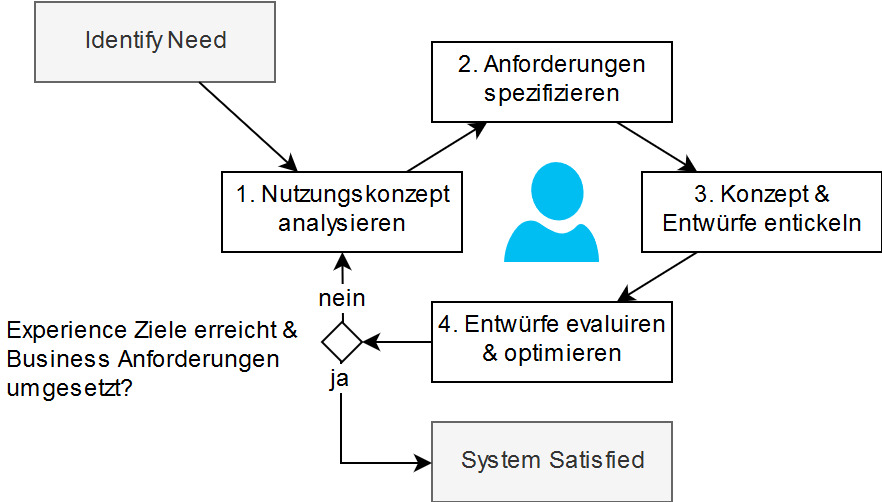
\includegraphics[keepaspectratio,width=0.8\textwidth]{UserCenteredDesign}
	\caption{Phasenmodell des ISO Standart 9241-210:2010 \parencite{ISO9241}}
\end{figure}

Um eine möglichst optimale User Experience zu erreichen, kann nach den Methodiken des Standards ISO 9241-210:2010 (fortan als User Centered Design bezeichnet) vorgegangen werden. Dies ist ein iteratives Vorgehen, bei dem die Benutzer im Zentrum stehen. Dies mit ihren Zielen, Bedürfnissen und Erwartungen über den gesamten Entwicklungsprozess hinweg. 
Jede Iteration dieses Prozesses durchläuft vier Phasen, bevor das Produkt in eine finale Version kommt.

Diese Methodik für die Ermittlung einer guten User Experience kann auch bei der Entwicklung einer AR Applikation verwendet werden.
In Phase 3 werden im User Centered Design zu Beginn meist Prototypen auf Papier entwickelt, mit welchem sich der Benutzter konzeptuell durch die Applikation navigieren muss. Diese Papierprototypen sind für eine dreidimensionale Applikation schwieriger zu gestalten und erschweren dadurch den Prozess. Bedingt durch diese Komplikation, ist der ganze Ablauf des User Centered Design teurer und komplexer (\cite{ISO9241}).

\subsection{Graphical User Interface Konzepte}
Im Rahmen des User Centered Designs gibt es zudem Richtlinien und Verhaltensweisen der graphischen Benutzeroberfläche.
Auch hier gilt, was bei zweidimensionalen GUI's funktioniert, muss nicht oder kann nicht zwingend bei einer AR Applikation verwendet werden. Um dem Benutzer die Interaktion mit der AR Applikation möglichst einfach und intuitiv zu gestalten, müssen folgende Punkte mit Sicherheit beachtet werden.

\subsubsection{Bildschirmflächenoptimierung}
Eine AR Applikation vermittelt den Eindruck, als ob die physikalische Welt die Limitierung der Applikation sei, in Wahrheit ist jedoch der Bildschirm des Anzeigegerätes die eigentliche Limitierung .
Der Benutzer möchte also möglichst wenig von seiner eigentlichen Intention, zum Beispiel der Besichtigung eines Gebäudes von aussen, abgelenkt werden. Dies setzt voraus, dass die Informationen sowie Interaktionsmöglichkeiten weitgehendst konsolidiert werden.

\subsubsection{Vereinfachter Einstieg}
Selbst in einer zweidimensionalen Applikation ist die Einarbeitung in eine Applikation teilweise sehr schwierig und zeitaufwendig. In einer dreidimensionalen Applikation gestaltet sich dies jedoch noch um einiges schwieriger und ist meist mit einer grösseren Lernkurve verbunden, weshalb der Einstieg ein noch wichtigerer Aspekt bei der Entwicklung sein muss.

\subsubsection{Vorhersehbarkeit}
Ein Benutzer bringt durch seine Bildung wie auch seine Herkunft schon Erwartungen mit. Diese antrainierte Verhalten sollte eine Applikation wo immer möglich nutzen und sinnvoll wiederverwenden. Als antrainiertes Verhalten gelten zum Beispiel Gesten zur Vergrösserung und Rotation einer Anzeige. Wo immer möglich sind solche intuitiven Verhalten einer Interaktion durch Buttons und Menüs vorzuziehen,

\subsubsection{Hinweise}
Der Mensch sucht stets nach Hinweisen und Signalen. Dieses Verhalten widerspiegelt sich auch in alltäglichen Situationen wie beispielsweise einer Bahnfahrt, auf welcher wir stets nach Symbolen und Hinweise für die Nächste Haltestelle oder Ausfahrt Ausschau halten.
Solche Hinweise sollen in einer AR Applikation den Benutzer ermutigen die Applikation noch weiter zu erkunden.
Diese Hinweise müssen nicht zwingend Texte sein, so kann auch ein Pfeil in die Richtung deuten, in welche sich das anzuzeigende Objekt befindet, sobald dieses aus dem Bildschirm tritt.

\subsubsection{Vielfältige Benutzer}
Eine AR Applikation soll stets für eine Vielzahl von Benutzer brauchbar sein. Dies soll besonders berücksichtigt werden. Es soll dabei Acht auf Behinderungen wie Farbenblindheit oder ähnliche Konditionen gegeben werden (\cite{AppleGuideline2018}, \cite{GoogleGuideline2018}, \cite{GoogleIO2018}, \cite{BerfinAyhan2017}).

\chapter{Ideen und Konzepte}

\chapter{Methode}

\section{Vorgehensmodell}

Alle Wirtschaftstprojekte an der Hochschule Luzern fallen in eine der folgenden Kategorien:

\begin{enumerate}
	\item Einsatz von Standardsoftware und Services
	\item Software- und Produktentwicklung
	\item Innovationsprojekt
	\item IT-Infrastrukturentwicklung
	\item Strukturierte Analyse und Konzeption von Systemen und Abläufen
\end{enumerate}

Dabei ist dieses Projekt als Innovationsprojekt und Softwareentwicklung klassifiziert worden. Wir erwarteten daher unter anderem, eine Evaluation, Recherchen und weitere Unbekannten. Um auf diese eingehen zu können, entschied sich das Team darauf die hybride, inkrementelle Agile Methode zu verwenden.

\subsection{Agile Projektmethode}

Die agile Projektmethode zielt darauf ab in einem ungewissen und sich verändernden Umfeld zu bestehen. Insbesondere heisst das, das auf sich verändernden Voraussetzungen schnell reagiert werden kann und ein funktionierendes Produkt dabei entsteht \parencite{AgileAlliance2015}. Dies soll durch eine enge Zusammenarbeit mit dem Auftraggeber und guter teaminterner Kommunikation erreicht werden.

Ein Rahmenplan dient als Richtschnur des Projektes, während die Anforderungen in den jeweiligen Sprints spezifiziert werden, und in der Sprintplanung festgehalten wird. Wir unterteilten unser Projekt in eine zweiwöchige Initialisierung, zweiwöchige Evaluation, und fünf Sprints in der unser Produkt entwickelt wurde.

\section{Anforderungsanalyse}


\section{Systemspezifikation}

\subsection{Systemübersicht}

\subsection{Architektur \& Design}
Die Architektur des Projektes wurde in 3 Schichten aufgeteilt. Diese werden in der nachfolgenden Grafik dargestellt. Dabei wurde ein Klassendiagramm erstellt, da es gleich den kompletten Aufbau des Projektes aufzeigt, sowie dessen Abhängigkeiten zu Schnittstellen (in der Grafik \textquoteleft Interfaces\textquoteright\ genannt).

\begin{figure}[h!]
	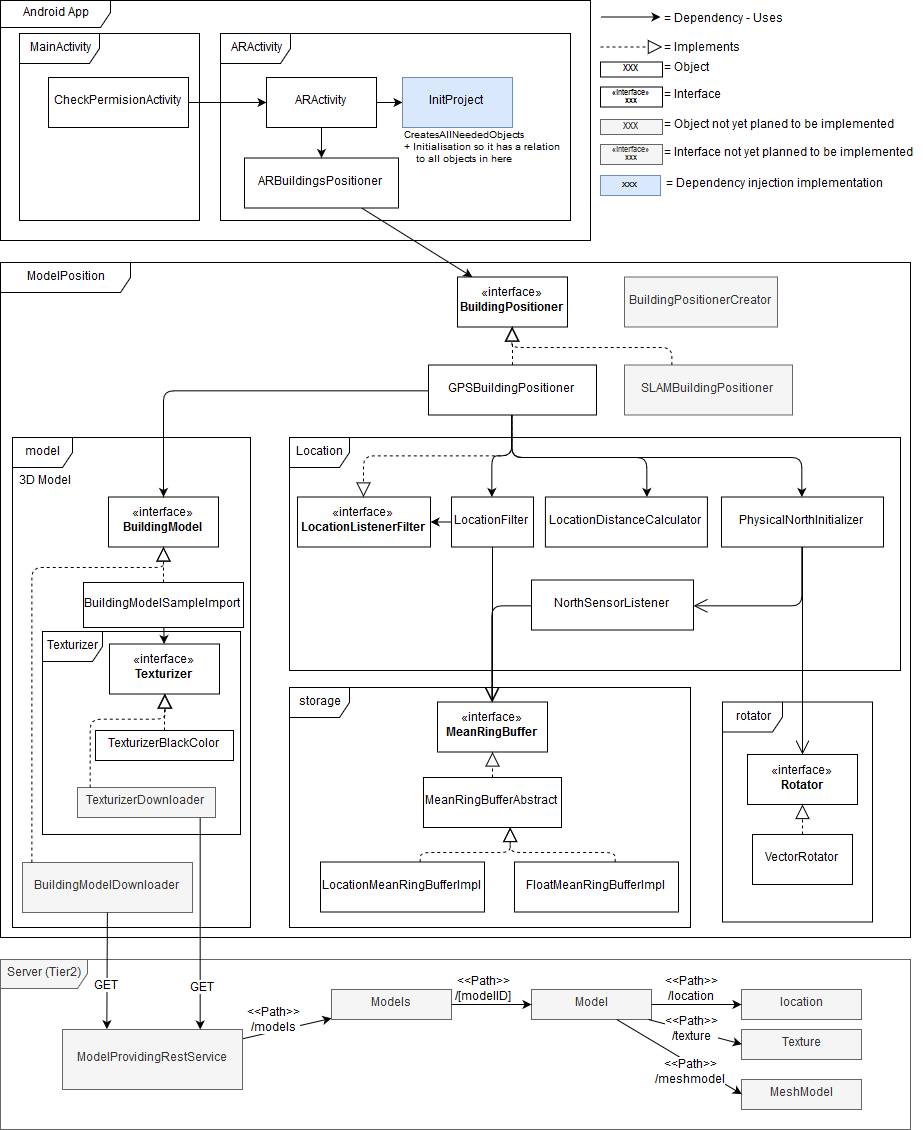
\includegraphics[keepaspectratio, width=\textwidth]{ArchitekturOverview.png}
	\caption{Architekturübersicht als Klassendiagramm}
\end{figure}

Eine detaillierte Beschreibung der einzelnen Schichten ist in den folgenden Kapiteln zu finden.

\begin{figure}[h!]
  \center
  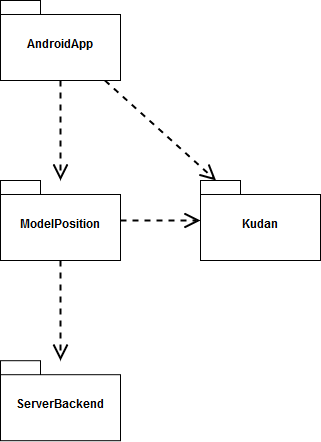
\includegraphics[width=0.35\textwidth]{SchichtenDiagramm.png}
  \caption{Übersicht der simplifizierten Schichtenarchitektur}
\end{figure}

\subsubsection{AndroidApp}
In AndroidApp befindet sich die kompletten graphischen Elemente der Applikation. Dies ist das Interface mit welchem der User arbeitet. Zudem werden hier die benötigten Berechtigungen geprüft und wenn nötig vom Benutzer erfragt.

\subsubsection{ModelPosition}
In ModelPosition ist die gesamte Logik für die Positionierung eines Gebäudes in der virtuellen Kudan Welt enthalten. Es abstrahiert zudem die Zugriffe auf Kudan selber, so dass diese nicht in der eigentlichen AndroidApp Komponente zu finden sind.

\subsubsection{Server}
Der Server ist eine über eine Rest Schnittstelle ansprechbare Komponente, welche das dynamische Laden von neuen Gebäuden ermöglicht. Diese ist ausserhalb dieses Projektscopes, wurde aus Gründen der Vollständigkeit jedoch dokumentiert und spezifiziert.

\subsection{Schnittstellen}
\subsubsection{Externe Schnittstellen}
Neben der Android Bibliothek wurde lediglich KudanAR als externe Schnittstelle verwendet. Die Dokumentation zu dieser Schnittstelle für Android ist unter folgendem Link zu finden:
\href{https://www.kudan.eu/docs-reference/AndroidDocs/annotated.html}{Dokumentation Kudan - Android}


\subsubsection{Interne Schnittstellen}

Die BuildingPositioner Schnittstelle ist verantwortlich für die Abstraktion des gesamten Positionierungsprozesses zur Applikation. Es bietet zudem Methoden an, welche dem Starten und Stoppen des Prozesses dienen.
\begin{figure}[h!]
	\center
	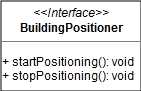
\includegraphics[scale=0.6]{BuildingPositioner.png}
	\caption{BuildingPositioner Interface}
\end{figure}
\clearpage
Das Building Model Interface ist das Bindeglied zwischen der realen Position des Benutzers und der virtuellen Position in der Applikationswelt. Es ist verantwortlich, dass das Gebäude reale Positionsdaten besitzt und die virtuellen Koordinaten an das Modell in der virtuellen Welt übergibt.

\begin{figure}[h!]
	\center
	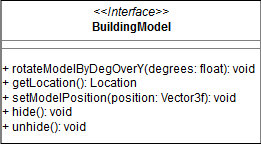
\includegraphics[scale=0.6]{BuildingModel.png}
	\caption{Building Model Interface}
\end{figure}

Der Texturizer ist verantwortlich für die Einfärbung des Modelles.
\begin{figure}[h!]
	\center
	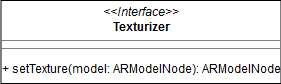
\includegraphics[scale=0.6]{Texturizer.png}
	\caption{Texturizer Interface}
\end{figure}


Der Rotator verpflichtet sich ein Rotating Object in einem Raum um eine bestimmte Achse zu drehen.
\begin{figure}[h!]
	\center
	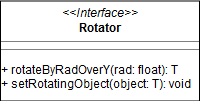
\includegraphics[scale=0.6]{Rotator.png}
	\caption{Rotator Interface}
\end{figure}


Der Mean Ring Buffer ist verantwortlich, dass ein Mittelwert eines Objektes <T> aus den übergebenen Objekten berechnet wird.
\begin{figure}
	\center
	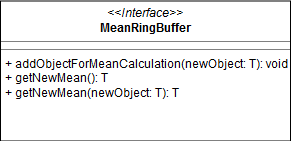
\includegraphics[scale=0.6]{MeanRingBuffer.png}
	\caption{Mean ring buffer Interface}
\end{figure}

\subsection{Anforderungen}

\subsection{Anwendung}

\section{Systemarchitektur}

\newpage
\section{Komponentendesign}

\begin{figure}[h!]
	\centering
	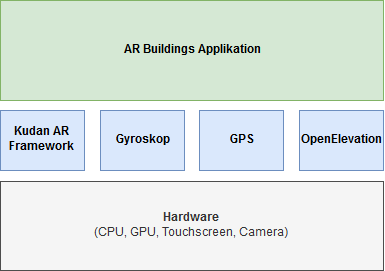
\includegraphics[width=0.7\linewidth, keepaspectratio]{Komponentendesign}
	\caption{Komponentendesign der ARBuildings Applikation}
\end{figure}

\section{Umsetzung Programmierung}

\section{Testing}

\subsection{Testplan}

\subsection{Testfälle}
\subsubsection{Testfall 1-Berechtigung erlauben}
\begin{tabularx}{\textwidth}{|l|X|}
\hline 
	Version &
	T-001v1 \\ 
\hline 
	Beschreibung & Berechtigungsanfragen \\ 
\hline 
	Testvoraussetzung & Die App hat die Berechtigungen noch nicht. \\ 
\hline 
	Testschritte &
		1. App starten \\ &
		2. Berechtigungen geben \\
\hline
	Erwartetes Ergebnis & Nachdem alle Berechtigungen gegeben wurden, startet die App wie gewollt \\ 
\hline 
\end{tabularx}
\subsubsection{Testfall 2-Berechtigung verweigern}
\begin{tabularx}{\textwidth}{|l|X|}
\hline 
	Version &
	T-002v1 \\ 
\hline 
	Beschreibung & Berechtigungsanfragen verweigern \\ 
\hline 
	Testvoraussetzung & Die App hat die Berechtigungen noch nicht. \\ 
\hline 
	Testschritte &
		1. App starten \\ &
		2. Berechtigungsanfragen sehen und ablehnen \\
\hline
	Erwartetes Ergebnis & Nachdem alle Berechtigungen nicht gegeben wurden, bleibt die App in einem Abfangbildschirm, wo die Nachfrage für die Berechtigungen erneut gestartet werden kann. \\ 
\hline 
\end{tabularx}
\subsubsection{Testfall 3-Starten von Kudan}
\begin{tabularx}{\textwidth}{|l|X|}
\hline 
	Version &
	T-003v1 \\ 
\hline 
	Beschreibung & 
	Es soll überprüft werden ob die Kudan Komponenten starten\\ 
\hline 
	Testvoraussetzung &
	T-001 wurde durchgeführt (Berechtigungen erhalten). \\ 
\hline 
	Testschritte &
		1. App starten \\
\hline
	Erwartetes Ergebnis &
	Es soll der Kamerabildschirm angezeigt werden. \\ 
\hline 
\end{tabularx}
\subsubsection{Testfall 4-Darstellung des Gebäudes Ausrichtung Norden}
\begin{tabularx}{\textwidth}{|l|X|}
\hline 
	Version &
	T-004v1 \\ 
\hline 
	Beschreibung & 
	Bei diesem Testfall soll getestet werden, ob das Gebäude Dargestellt wird.\\ 
\hline 
	Testvoraussetzung &
	Die App ist auf dem Smartphone installiert. GPS gemocked auf folgende Position: \\ & 
		47.145739885261925,8.436641571608824, Altitude: 450 \\ 
\hline 
	Testschritte & 
		1. Smartphone nach norden ausrichten \\ &
		2. App starten \\ &
		3. Initialisierung abwarten (ca. 3 Sekunden)\\
\hline
	Erwartetes Ergebnis &
	Das Gebäude wird auf 7Uhr 30 dargestellt. \\ 
\hline 
\end{tabularx}
\subsubsection{Testfall 5-Darstellung des Gebäudes Ausrichtung Westen}
\begin{tabularx}{\textwidth}{|l|X|}
\hline 
	Version &
	T-005v1 \\ 
\hline 
	Beschreibung & 
	Bei diesem Testfall soll getestet werden, ob das Gebäude Dargestellt wird wenn es nicht nach norden gerichtet ist. \\ 
\hline 
	Testvoraussetzung &
	Die App ist auf dem Smartphone installiert. GPS gemocked auf folgende Position: \\ &
		47.145739885261925,8.436641571608824, Altitude: 450 \\ 
\hline 
	Testschritte & 
		1. Smartphone nach Westen ausrichten \\ &
		2. App starten \\ &
		3. Initialisierung abwarten (ca. 3 Sek) \\
\hline
	Erwartetes Ergebnis &
	Das Gebäude wird auf 10Uhr 30 dargestellt. \\ 
\hline 
\end{tabularx}
\subsubsection{Testfall 6-Darstellung Gebäude mit Bewegung nach rechts}
\begin{tabularx}{\textwidth}{|l|X|}
\hline 
	Version &
	T-006v1 \\ 
\hline 
	Beschreibung & 
	Bei diesem Testfall soll getestet werden, ob das Gebäude dargestellt wird und sich die Position des Gebäudes den GPS Daten anpasst. \\ 
\hline 
	Testvoraussetzung &
	Die App ist auf dem Smartphone installiert. GPS gemocked auf folgende Position: \\ &
		47.145739885261925,8.436641571608824, Altitude: 450 \\ 
\hline 
	Testschritte & 
		1. Smartphone nach Westen ausrichten \\ &
		2. App starten \\ &
		3. 3 Sekunden warten \\ &
		4. App minimieren (Home Button drücken) \\ &
		5. GPS Mocklocation verändern (auf Position 47.145739885261925,8.436641571608824) \\ &
		6. App erneut öffnen \\
\hline
	Erwartetes Ergebnis &
	Das Gebäude wandert von 10Uhr 30 auf 12Uhr \\ 
\hline 
\end{tabularx}
\subsubsection{Testfall 7-Darstellung Gebäude mit Bewegung nach links}
\begin{tabularx}{\textwidth}{|l|X|}
\hline 
	Version &
	T-007v1 \\ 
\hline 
	Beschreibung & 
	Bei diesem Testfall soll getestet werden, ob das Gebäude dargestellt wird und sich die Position des Gebäudes den GPS Daten anpasst. \\ 
\hline 
	Testvoraussetzung &
	Die App ist auf dem Smartphone installiert. GPS gemocked auf folgende Position: \\ &
		47.142958, 8.430126, Altitude: 450 \\ 
\hline 
	Testschritte & 
		1. Smartphone nach Norden ausrichten \\ &
		2. App starten \\ &
		3. 3 Sekunden warten \\ &
		4. App minimieren (Home Button drücken) \\ &
		5. GPS Mocklocation verändern (auf Position  47.141427, 8.432621) \\ &
		6. App erneut öffnen \\
\hline
	Erwartetes Ergebnis &
	Das Gebäude wandert von 15Uhr auf 12Uhr \\ 
\hline 
\end{tabularx}
\subsubsection{Testfall 7-Darstellung Gebäude mit Bewegung nach links}
\begin{tabularx}{\textwidth}{|l|X|}
\hline 
	Version &
	T-007v1 \\ 
\hline 
	Beschreibung & 
	Bei diesem Testfall soll getestet werden, ob das Gebäude dargestellt wird und sich die Position des Gebäudes den GPS Daten anpasst. \\ 
\hline 
	Testvoraussetzung &
	Die App ist auf dem Smartphone installiert. GPS gemocked auf folgende Position: \\ &
		47.142958, 8.430126, Altitude: 450 \\ 
\hline 
	Testschritte & 
		1. Smartphone nach Norden ausrichten \\ &
		2. App starten \\ &
		3. 3 Sekunden warten \\ &
4. App minimieren (Home Button drücken) \\ &
		5. GPS Mocklocation verändern (auf position  47.141427, 8.432621) \\ &
		6. App erneut öffnen \\
\hline
	Erwartetes Ergebnis &
	Das Gebäude wandert von 15Uhr auf 12Uhr \\ 
\hline 
\end{tabularx}
\subsubsection{Testfall 8-Entfernen der Berechtigung zur Laufzeit}
\begin{tabularx}{\textwidth}{|l|X|}
\hline 
	Version &
	T-008v1 \\ 
\hline 
	Beschreibung & 
	Bei diesem Testfall so überprüft werden ob die App nicht abstürzt, wenn zur Laufzeit der App Berechtigungen entzogen werden. \\ 
\hline 
	Testvoraussetzung &
	Die App ist auf dem Smartphone installiert und hat alle nötigen Berechtigungen \\ 
\hline 
	Testschritte & 
		1. App starten \\ &
		2. App minimieren \\ &
		3. Berechtigungen der App entfernen \\ &
		4. App wieder öffnen \\
\hline
	Erwartetes Ergebnis &
	Die App schaltet wieder auf den Berechtigungsbildschirm. \\ 
\hline 
\end{tabularx}
\subsubsection{Testfall 9-Smartphone Rotation}
\begin{tabularx}{\textwidth}{|l|X|}
\hline 
	Version &
	T-009v1 \\ 
\hline 
	Beschreibung & 
	Es soll überprüft werden wie das Verhalten ist, wenn das Smartphone rotiert wird. \\ 
\hline 
	Testvoraussetzung &
	Die App hat alle Berechtigungen \\ 
\hline 
	Testschritte & 
		1. App starten \\ &
		2. 3 Sekunden warten \\ &
		3. Rotieren des Smartphones um 90 grad (Portrait auf Landscape) \\
\hline
	Erwartetes Ergebnis &
	Die App soll keine Rotationsanimation beinhalten. Die App soll das Gebäude weiter anzeigen. \\ 
\hline 
\end{tabularx}

\chapter{Realisierung}

% TODO Ein Beispiel für den Gebrauch von Formeln und Referenz auf die jeweilige Formel - entfernen wenn nicht mehr gebraucht
Die Distanz zwischen zwei Geopositionen wird über die Bogenlänge (siehe \ref{Bogenlaenge}) der Differenz der Längen- und Breitengrade ausgerechnet.

\indexequation{b = \frac{\pi}{\SI{180}{\degree}}\beta r}{Bogenlänge des Winkels $\beta$ mit Radius $r$}{Bogenlaenge}

\section{Ermittlung offener Projektrahmenbedingungen}
\label{sec:evaluation}
Im Rahmen dieses Projektes mussten verschiedene Unbekannte zuerst analysiert und evaluiert werden. Dazu gehörten die Zielplattform, Entwicklungsumgebung und die zu verwendenden Augmented Reality Frameworks.
\subsubsection{Zielplattform}
Als Zielplattform standen gemäss Projektbeschrieb die Folgenden zur Auswahl:
\begin{itemize}
\item Microsoft HoloLens
\item Smartphone und Tablets
\end{itemize}
Für alle dieser Plattformen galt die Idee, diese als Interface zu gebrauchen um das AR Gebäude in der Umgebung anzuzeigen. Alle drei Zielplattformen weisen unterschiedliche Stärken und Schwächen auf.

Die HoloLens zeigte grosse Schwächen beim Gebrauch im Freien, da deren Bildschirm für den Aussengebrauch zu wenig Hell ist. Zudem fehlen der HoloLens Lokalisierungssensoren. Im Rahmen einer Analyse der Bedienung wurden 5 Probanden dazu aufgefordert mit der vorhanden HoloLens und HoloLens Apps zu interagieren, und ihr Verhalten beobachtet. Die Probanden besassen keinerlei Erfahrung im Umgang mit der HoloLens und es wurde ihnen auch keine vorgängigen Informationen zur Bedienung mitgeteilt. Bei diesem Test stellte sich heraus, dass die Interaktion mit der HoloLens für alle Probanden nicht intuitiv war. Dies äusserte sich in Gesten die von der HoloLens nur manchmal erkannt wurden (Pinching) und solche die zwar für Probanden intuitiv waren, aber von der Hololens ignoriert wurden (antippen eines virtuellen Objektes).
Das Positive der HoloLens ist die nahtlose Integration der Augmented Reality Modelle in die Umgebung des Betrachters. 
 
Die Smartphones zeigen ihre grosse Stärke in der Verbreitung. Dies führt zu einer hohen Vertrautheit des Benutzers mit dem Gerät. Zudem sind die heutigen Smartphones hell genug um das Display bei normalen Tageslicht zu sehen.
Nachteile zeigen sich in der Haltung des Gerätes, da für die Einbindung der Augmented Reality Modelle das Smartphone ständig in den Händen gehalten werden muss.

In einer ersten Evaluation mit einer Hololens wurde entschieden, dass für dieses Projekt die Hololens ausgeschlossen werden soll, da diese für Ausseneinsätze nur bedingt verwendet werden kann.

Dank der Höheren Verbreitung und der damit entstehenden höheren Flexibilität beim entwickeln, fiel die Entscheidung auf eine Smartphonelösung. Es wurde schliesslich noch auf die Android Plattform eingeschränkt, dies aus den Gründen, dass Android keine speziellen Bedingungen voraussetzt und somit auch auf den bereits vorhanden Geräten verwendet werden kann. 

\subsubsection{Entwicklungsumgebung}
\label{ssec:EvalPlattform}
Bedingt durch die Selektion der Zielplatform standen verschiedene Entwicklungsumgebungen zur Verfügung. Dabei wurden folgende zwei Entwicklungsumgebungen miteinander verglichen:
\begin{itemize}
\item Unity
\item AndroidStudio
\end{itemize}

Auf beiden Entwicklungsumgebungen wurde ein Prototyp für Android entwickelt. Dabei entstand folgende Auffassung:

Bei Unity ist das Erstellen einer ersten lauffähigen Version sehr einfach. Ein weiterer Vorteil ist die grafische Darstellung der 3D Modelle. Zudem würde eine allfällige Portierung auf weitere Platformen einfach umsetzbar sein. Bei der Entwicklung stellte sich eine Schwäche mit den GPS Sensoren heraus. So funktionierten diese aus unbekannten Gründen nicht bei jeder Installation der Applikation korrekt. Für die Lösung dieses Problemes fehlte eine ausreichende Debugmöglichkeit in Unity.

Android Studio zeigte seine Stärke in den Debugmöglichkeiten und der ausgezeichneten API Dokumentation. So funktionierten alle benötigten Sensoren auf Anhieb. Die Schwächen dieser Entwicklungsumgebung liegt darin, dass eine allfällige Portierung auf weitere Plattformen nur durch eine Neuimplementation möglich ist. Zudem werden die 3D Modelle nicht grafisch dargestellt und müssen mit einer anderen Software Editiert werden.

Die unzureichende Debugmöglichkeiten sowie die Problemen mit den GPS Sensoren waren die Hauptgründe die Unity Entwicklungsumgebung nicht für die Implementation zu gebrauchen.

\subsubsection{Augmented Reality Frameworks}
Während der Recherchen stellte sich heraus, dass ein breites Spektrum verschiedener AR Frameworks auf dem Markt vorhanden ist. Jedes Framework setzt dabei auf eigene Anwendungsbereiche. Für dieses Projekt wurden vier häufig verwendete und gut dokumentierte Frameworks näher untersucht (\cite{DDIDevelopment}). Konkret handelte es sich dabei um folgende Frameworks:
\begin{itemize}
\item Kudan
\item Vuforia
\item Wikitude
\item ARtoolKit
\end{itemize}

Die Folgende Tabelle zeigt eine vereinfachte Darstellung der 4 Frameworks. Sie vergleicht die für dieses Projekt notwendigen Features, sowie die Lizenzierung (\cite{DDIDevelopment}).

\begin{table}[h!]
	\center
	\begin{tabular}{|c|c|c|c|c|}
		\hline 
		& \textbf{Mobile} & \textbf{UWP (Hololens)} & \textbf{SLAM} & \textbf{Licence} \\ 
		\hline 
		Kudan & \checkmark & x & \checkmark & Commercial, free \\ 
		\hline 
		Vuforia & \checkmark & \checkmark & \checkmark & Commercial \\ 
		\hline 
		Wikitude & \checkmark & \checkmark & \checkmark & Commercial, free \ \\ 
		\hline 
		ARToolkit & \checkmark & x & x & OpenSource \\ 
		\hline 
	\end{tabular}
	\caption{Vergleichstabelle verschiedener AR Frameworks}
\end{table}


Für das Projekt wurde entschieden Kudan als AR Framework zu verwenden. Gründe dafür lagen darin, dass dieses Framework über eine sehr robuste single-Kamera SLAM Implementation verfügt (\cite{BerfinAyhan2017}), und das Lizenzierungsmodell, welche eine Entwicklung ohne weitere Kosten ermöglichte. Der wichtigste Grund lag jedoch darin, dass die Dokumentation sehr extensiv, und die Erfahrung mit Kudan am Grössten war.

\section{Einschränkungen und Abgrenzungen}

Wie aus der Evaluation (siehe \ref{ssec:EvalPlattform}) ersichtlich ist, haben wir uns schlussendlich auf Android als Plattform beschränkt. Dies hat zur Folge das der erarbeitete Code nicht ohne weiteres auf andere Plattformen portiert werden kann. Die Architektur ist aber so modular aufgebaut, dass die Implementierung für andere Plattformen dennoch ohne grossen Aufwand geschehen kann.

Weiter haben wir die Androidversion auf Version 6.0 und aufwärts eingeschränkt. Dies entspricht etwa 80\% aller Androidbesitzer (siehe Abb. \ref{fig:AndroidMarketshare}), und beinhaltet wichtige Funktionen die wir für unser Projekt gebrauchen. Zudem muss das jeweilige Gerät folgende Systemanforderungen besitzen:
\begin{itemize}
	\item Gyroskop
	\item Magnetometer (Kompass)
	\item GPS Lokationssensor (GLOSNASS, GALILEO, BEIDU)
\end{itemize}

\begin{figure}
	\centering
	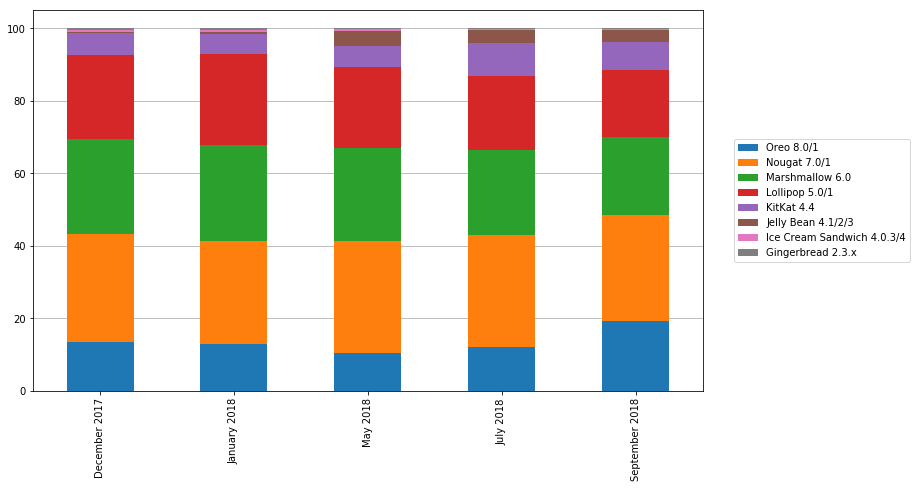
\includegraphics[keepaspectratio,width=0.8\textwidth]{AndroidMarketshare}
	\caption{Prozentanteil der Androidversionen, Daten von \cite{Fossbytes2018}}
	\label{fig:AndroidMarketshare}
\end{figure}


\newpage
\section{Projektmanagementplan}

\subsection{Projektorganisation}
Da beide Projektmitglieder ihre Kompetenzen eher in den technischen Bereichen dieses Projekts sehen, wurde von einer strikten Aufgabenteilung abgesehen.

Es wurde dennoch darauf geachtet, dass beide Mitglieder klare Verantwortungen übernehmen. Diese waren jedoch mehr in einer überwachenden Funktion gesehen, und soll nicht heissen, dass dieses Mitglied die Arbeit alleine leistete.

\vspace{1em}

\begin{tabularx}{\textwidth}{|X|X|}
	\hline
	\textbf{Teammitglied} & \textbf{Funktionen} \\
	\hline
	Pascal Baumann & \tabitem Dokumentation \\
	& \tabitem Testplanung \& Durchführung \\
	& \tabitem Projektmanagement \\
	\hline
	Dane Wicki & \tabitem Architektur \\
	& \tabitem Plattformanalyse \\
	\hline
\end{tabularx}

\newpage
\subsection{Projektführung}

\subsection{Rahmenplan}

Das Projekt wurde in 6 zweiwöchige Sprints unterteilt und in diesen iterativ entwickelt.

\vspace{1em}

\begin{figure}[h!]
	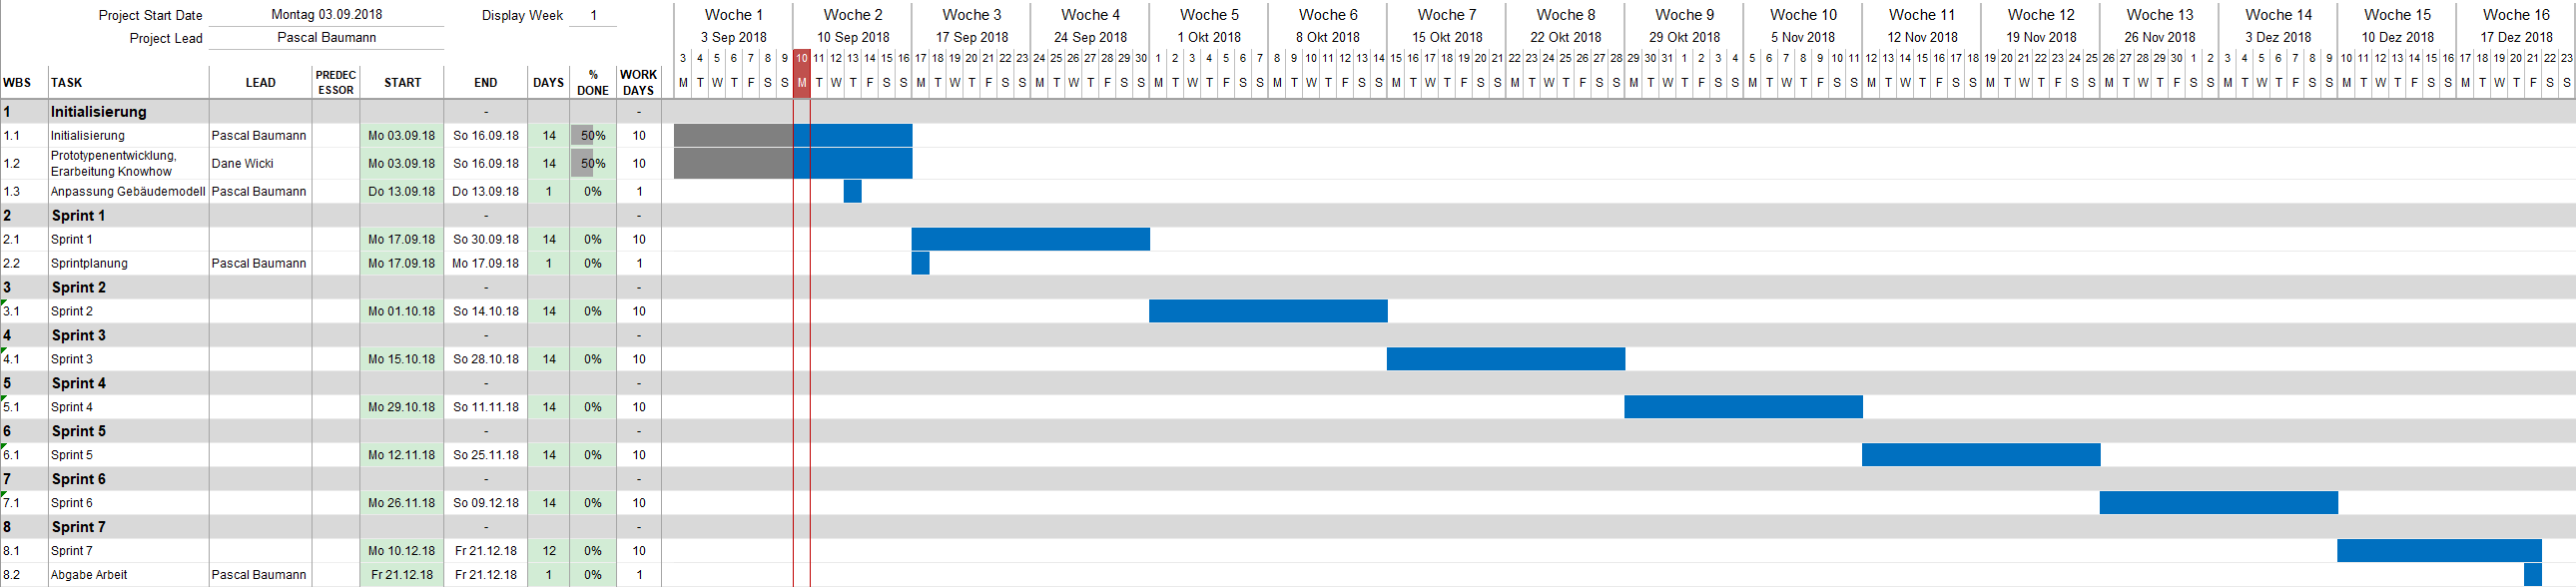
\includegraphics[keepaspectratio, width=\textwidth]{Rahmenplan}
	\caption{Überblick der Sprints}
\end{figure}

\subsection{Tools}
\label{sec:Tools}
\begin{table}[h!]
	\begin{tabular}{|p{0.4\textwidth}|p{0.6\textwidth}|}
		\hline
		\textbf{Aufgabe} & \textbf{Hilfsmittel} \\
		\hline
		Dokumente und Dokumentation & TeX / GitHub \\
		\hline
		Versionierung Dokumentation & git / GitHub\\
		\hline
		Dokumentation Code & JavaDoc \\
		\hline
		Git Clients & GitKraken, git Terminal\\
		\hline
		Quellen & Mendeley \\
		\hline
		Dateiablage für Teamaustausch & OneDrive \\
		\hline
		Rahmenplan & MS Excel 2016 \\
		\hline
		Kommunikation Team & WhatsApp\\
		\hline
		Aufgabenverwaltung & Trello, Rahmenplan\\
		\hline
		Entwicklungsumgebung Arduino & Arduino Studio\\
		\hline
	\end{tabular}
	\caption{Gebrauchte Software Hilfsmittel}
	\label{tab:SWTools}
\end{table}

\subsection{Risikomanagement}

Es werden mögliche Risiken welche während dem Projekt auftreten können aufgezählt. Diese werden auf Eintrittswahrscheinlichkeit und Schadensmass eingeschätzt, danach wird entschieden, welche Massnahmen getroffen werden können, und was deren Auswirkungen sind.

\subsubsection{Definitionen}
\label{sssec:Def}
\vspace{1em}
\noindent
Eintrittswahrscheinlichkeit:

\vspace{1em}
\noindent
\begin{tabular}{|p{0.06\textwidth}|p{0.2\textwidth}|p{0.7\textwidth}|}
	\hline
	\textbf{Stufe} & \textbf{Bezeichnung} & \textbf{Beschreibung} \\
	\hline
	1 & unvorstellbar & Möglich aber eher unwahrscheinlich. Tritt nie oder einmal in 14 Wochen auf \\
	\hline
	2 & unwahrscheinlich & Kann in 14 Wochen 1-5 Mal eintreten\\
	\hline
	3 & vorstellbar & Kann in 14 Wochen 6-8 Mal eintreten \\
	\hline
	4 & wahrscheinlich & Kann in 14 Wochen bis zu 10 Mal eintreten \\
	\hline
	5 & häufig & Kann in 14 Wochen 14 Mal eintreten\\
	\hline
\end{tabular}

\vspace{1em}
\noindent
Schadensausmass:

\vspace{1em}
\noindent
\begin{tabular}{|p{0.06\textwidth}|p{0.2\textwidth}|p{0.7\textwidth}|}
	\hline
	\textbf{Stufe} & \textbf{Bezeichnung} & \textbf{Beschreibung} \\
	\hline
	1 & unwesentlich & Die Aufgabenerfüllung wird höchstens geringfügig beeinträchtigt finanzieller Schaden ist im Rahmen des Projekts nicht beeinflussend. Personenschäden treten nicht auf \\
	\hline
	2 & geringfügig & Wahrnehmbare Gefährdung / Einfluss auf das Projekt. Personenschäden treten nicht auf \\
	\hline
	3 & mittelmässig & Wahrnehmbare Gefährdung / Einfluss auf das Projekt.Finanzieller Schaden strapaziert das Projektbudget
	Personenschäden treten nicht auf \\
	\hline
	4 & kritisch & Starke Gefährdung des Projekts. Finanzieller Schaden übersteigt das Projektbudget massiv. Personenschäden treten geringfügig auf \\
	\hline
	5 & katastrophal & Projektabbruch zur Folge. Finanzieller Schaden kann zum Projektstopp führen. Verletzung der Persönlichkeitsrechte
	\\
	\hline
\end{tabular}

\subsubsection{Risikokatalog}
\label{sssec:Risikokatalog}
Legende:
\begin{itemize}
	\item \textbf{S}chadensausmass bei Eintreffen des Risikos
	\item \textbf{W}ahrscheinlichkeit das Risiko eintrifft
	\item \textbf{K}ategorie: \textbf{T}echnisches oder \textbf{P}rojektbezogenes Risiko
	\item \textbf{A}uswirkung auf das Projekt. Produkt aus S und W
\end{itemize}

\vspace{1em}
\noindent
\begin{tabular}{|p{0.03\textwidth}|p{0.75\textwidth}|p{0.03\textwidth}|p{0.03\textwidth}|p{0.03\textwidth}||p{0.03\textwidth}|}
	\hline
	\textbf{Nr.} & \textbf{Beschreibung / Risiko} & \textbf{K} & \textbf{S} & \textbf{W} & \textbf{A} \\
	\hline
	1 & Datenverlust & P & 5 & 1 & 5\\
	\hline
	2 & Fehlkommunikation im Team & P & 3 & 2 & 6 \\
	\hline
	3 & Teammitglied fällt aus & P & 3 & 2 & 6 \\
	\hline
	4 & Verzug bei Erstellung von Dokumenten & P & 3 & 2 & 6 \\
	\hline
	5 & Prototyp entspricht nicht den Kundenwünschen & T & 5 & 2 & 10 \\
	\hline
\end{tabular}

\vspace{1em}

\begin{figure}[h!]
	\centering
	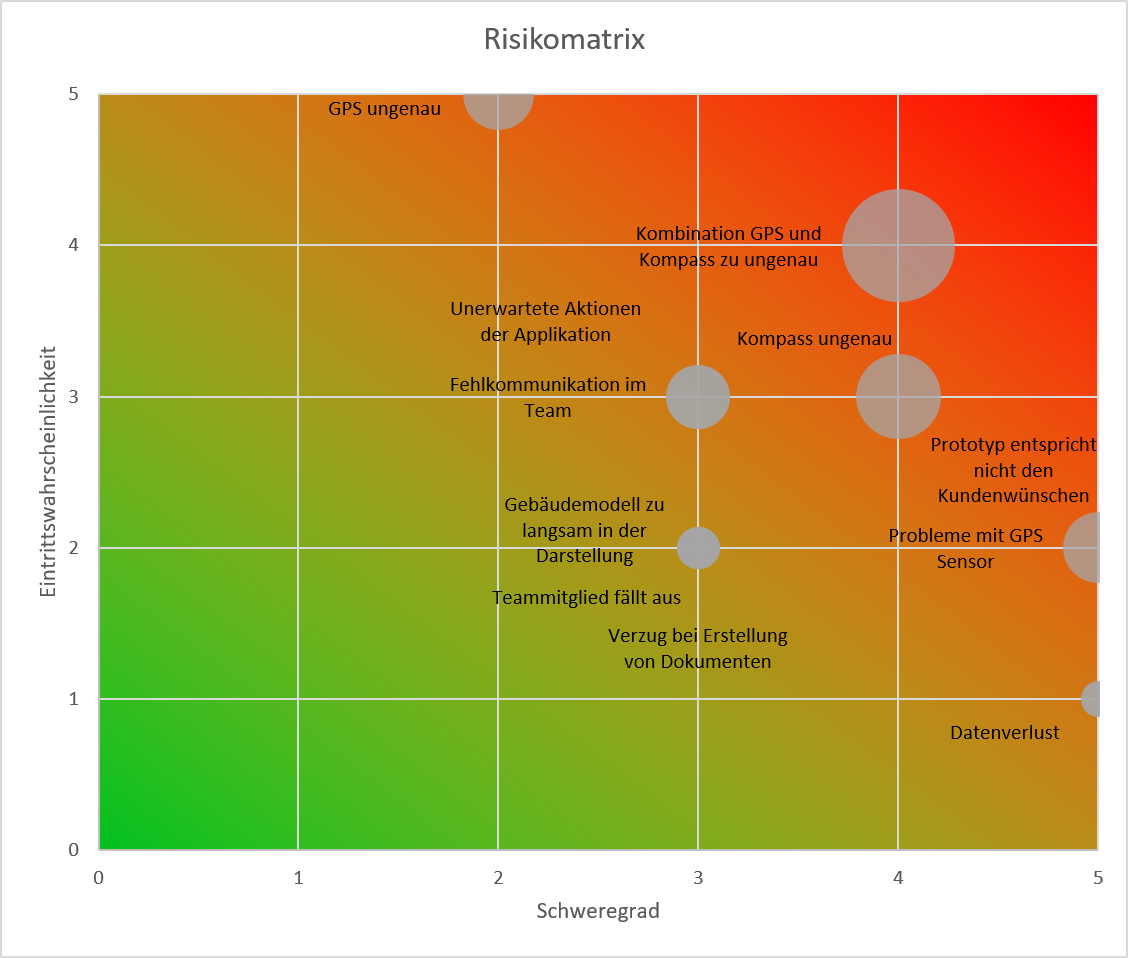
\includegraphics[keepaspectratio, width=0.8\textwidth]{RisikoMatrix}
	\caption{Auswirkungen der Risiken}
\end{figure}

\chapter{Evaluation und Validation}


\chapter{Ausblick}

\appendix

\chapter{Testprotokolle}


\glossary{Abkürzungsverzeichnis}

\listoffigures

\listoftables

\listofmyequations \pagebreak

\printbibliography

\chapter*{Eidesstattliche Erklärung}
Ich erkläre hiermit, dass ich/wir die vorliegende Arbeit selbständig und ohne unerlaubte fremde Hilfe angefertigt haben, alle verwendeten Quellen, Literatur und andere Hilfsmittel angegeben haben, wörtlich oder inhaltlich entnommene Stellen als solche kenntlich gemacht haben, das Vertraulichkeitsinteresse des Auftraggebers wahren und die Urheberrechtsbestimmungen der Fachhochschule Zentralschweiz (siehe Merkblatt «Studentische Arbeiten» auf MyCampus) respektieren werden.

\vspace{1em}

\renewcommand{\arraystretch}{2}
\begin{tabularx}{\textwidth}{XXXX}
	Unterschrift: & & Unterschrift: & \\ \cline{2-2}\cline{4-4}
	Baumann, Pascal & & Wicki, Dane & \\
	Datum: & & Ort: & \\
\end{tabularx}

\end{document}
